\chapter{The morphological dependance of quenching}

\emph{The work in the following chapter has been published in \citet{smethurst15}.}

\begin{figure}
\centering{
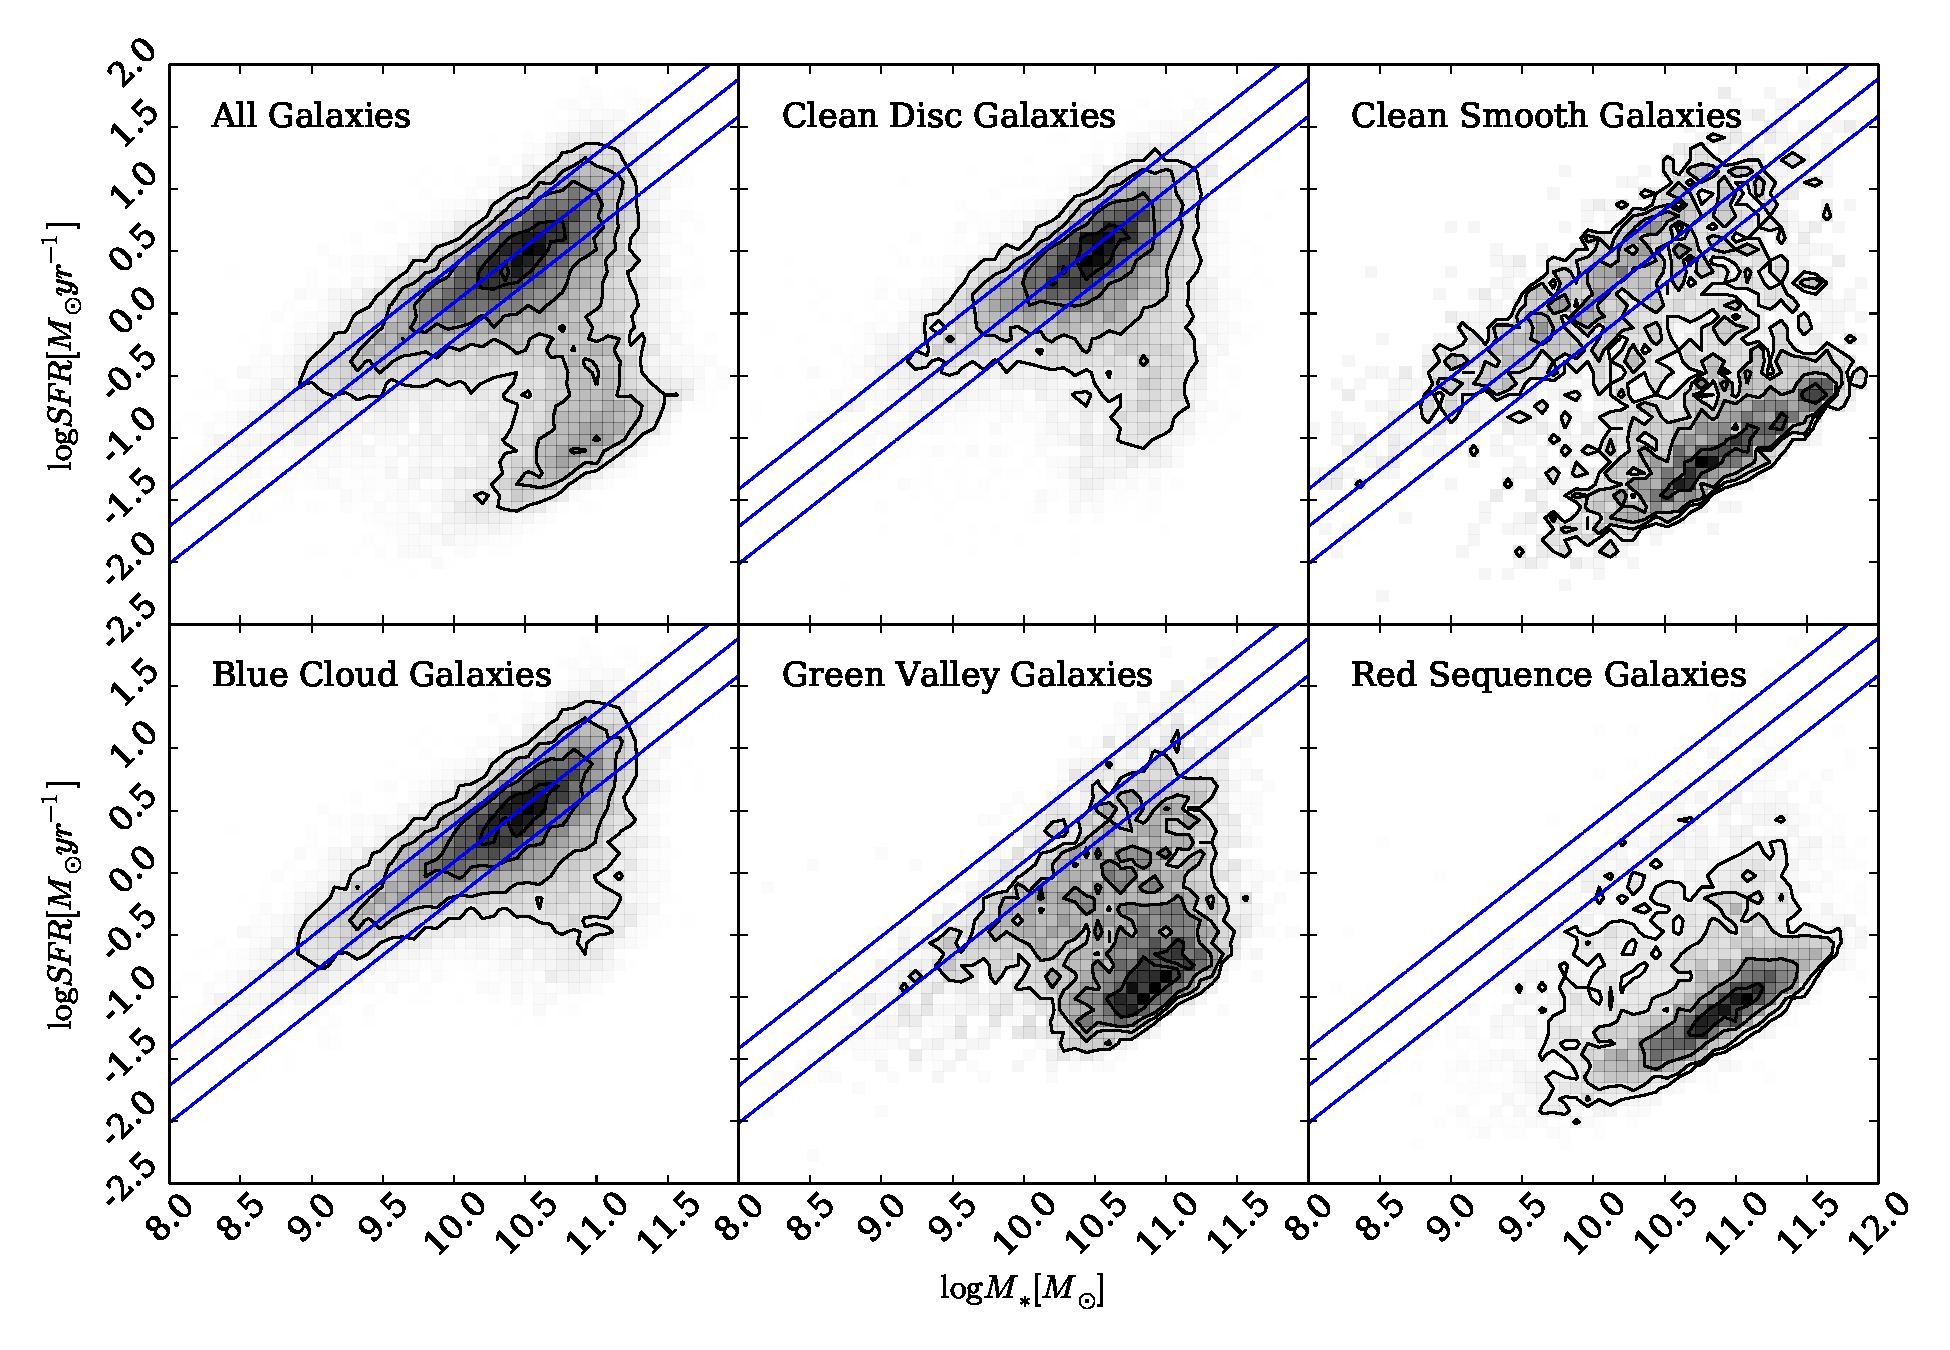
\includegraphics[width=\textwidth]{morphology/sfr_mass_subsets.pdf}}
\caption[SFR-stellar mass plane split by morphology and colour]{Star formation rate versus stellar mass diagrams show the different populations of galaxies  (top row, left to right: all galaxies, GZ2 `clean' disc and smooth galaxies; bottom row, left to right: blue cloud, green valley and red sequence galaxies) and how they contribute to the star forming sequence (from \citet{peng10}, shown by the solid blue line with 0.3 dex scatter by the dashed lines). Based on positions in these diagrams, the green valley does appear to be a transitional population between the blue cloud and the red sequence. Detailed analysis of star formation histories can elucidate the nature of the different populations' pathways through the green valley. The clean smooth and disc samples are described in Section~\ref{class}.}
\label{sfr_mass_sub}
\end{figure}

Figure~\ref{sfr_mass_sub} shows the SFR versus the stellar mass for the observed GZ2 sample which has been split into blue cloud, green valley and red sequence populations as well as into the `clean' disc and smooth galaxy samples (with GZ2 vote fractions of $p_d \geq 0.8$ and $p_s \geq 0.8$ respectively). The green valley galaxies are indeed a population which have either left, or begun to leave, the star forming sequence or have some residual star formation still occurring. 


The left panel in Figure~\ref{sfr_mass_col} shows a handful of quenching models and how they reproduce the observed relationship between the SFR and the mass of a galaxy, including how at the time of quenching they reside on the star forming sequence shown by the solid black line for a galaxy of mass, $M = 10^{10.27} M_{\odot}$.   The right panel shows how these SFRs translate into the optical-NUV colour-colour plane to reproduce observed colours of green valley and red sequence galaxies. Some of the SFHs produce colours redder than the apparent peak of the red sequence in the GZ2 subsample; however this is not the \emph{true} peak of the red sequence due to the necessity for NUV colours from GALEX (see Section \ref{class}). 

The majority of the red galaxies in the sample therefore lie towards the \emph{blue end} of the red sequence and have a small amount of residual star formation in order to be detected in the NUV resulting in a specific subset of the red sequence studied in this investigation. Only $47\%$ of the red sequence galaxies present in the entire Galaxy Zoo 2 sample are matched with GALEX to produce our final sample of $126, 316$ galaxies, as opposed to $72\%$ of the blue cloud and $53\%$ of the green valley galaxies. This limitation should be taken into account when considering the results in the following sections.

 The SFH models were implemented with the \starpy ~package to produce Figures~\ref{red_s},~\ref{green_v} \&~\ref{blue_c} for the red sequence, green valley and blue cloud populations of smooth and disc galaxies respectively. The percentages shown in Figures~\ref{red_s},~\ref{green_v} \&~\ref{blue_c} are calculated as the fractions of the combined posterior probability distribution located in each region of parameter space for a given population. 

Since the sample contains such a large number of galaxies, we interpret these fractions as broadly equivalent to the percentage of galaxies in a given population undergoing quenching within the stated timescale range. Although this is not quantitatively exact, it is nevertheless a useful framework for interpreting the results of combining the individual posterior probability distributions of each galaxy.

Also shown in Figure~11 are the median walker positions (the 50th percentile of the Bayesian probability distribution) of each individual galaxy, split into red, green and blue populations also with a hard cut in the vote fraction of $p_d > 0.5$ and $p_s > 0.5$ to show the disc and smooth populations respectively. These positions were calculated without discarding any walker positions due to low probability and without weighting by vote fractions; therefore this may be more intuitive to understand than Figures~\ref{red_s},~\ref{green_v} \&~\ref{blue_c}.

Although the quenching timescales are continuous in nature, in this Section we refer to rapid, intermediate and slow quenching timescales which correspond to ranges of  $\tau ~\rm{[Gyr]} < 1.0$, $1.0 < \tau ~\rm{[Gyr]} < 2.0$ and $\tau ~\rm{[Gyr]} > 2.0$ respectively for ease of discussion.



\section{The Red Sample}\label{rs}

\begin{figure*}
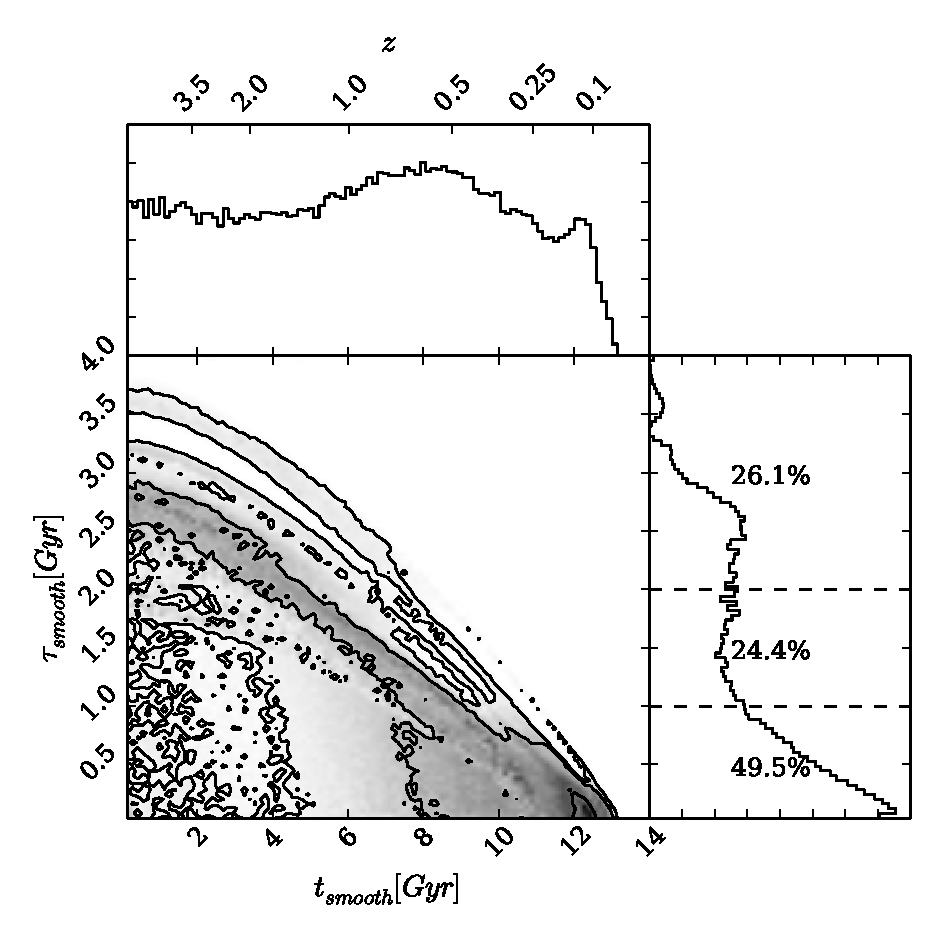
\includegraphics[width=0.4975\textwidth]{morphology/red_smooth.pdf}
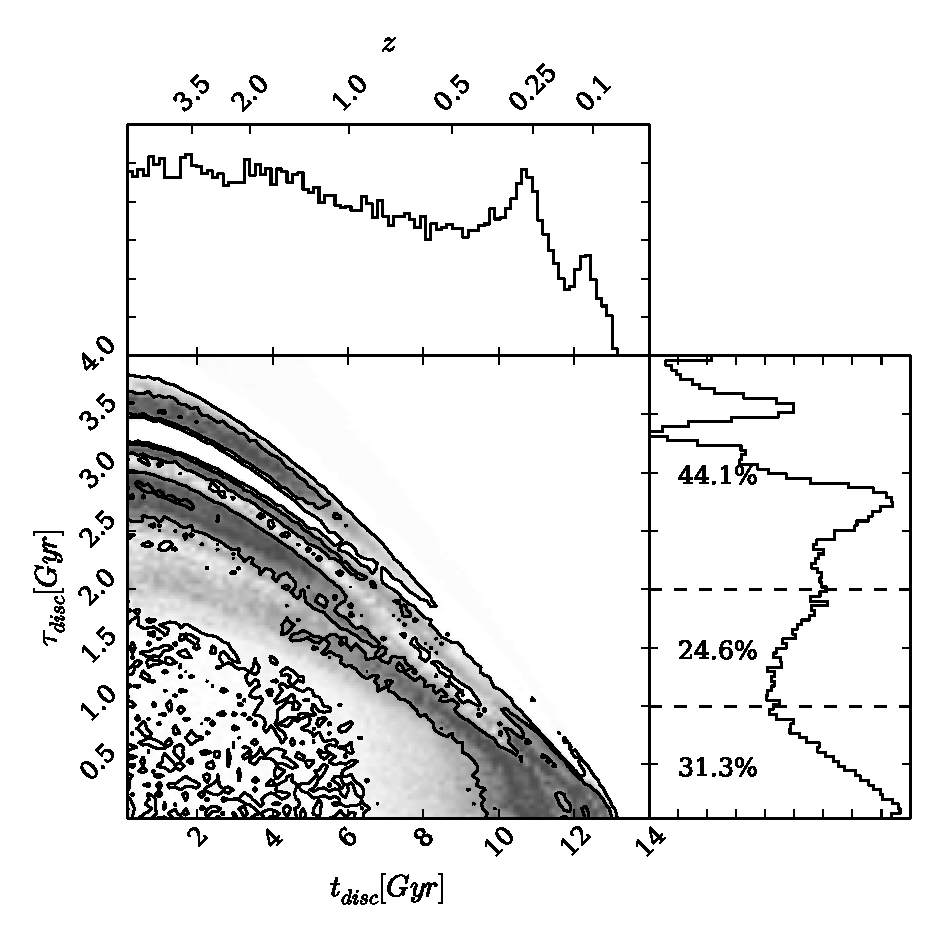
\includegraphics[width=0.4975\textwidth]{morphology/red_disc.pdf}
\caption[Population densities of red smooth and disc galaxies]{Contour plots showing the combined positions in the Markov Chain for all red galaxies in this study, weighted by the logarithmic probability of each position (see Section \ref{stats}) and also by the morphological vote fractions from GZ2 to give the areas of high probability in the model parameter space for both bulge (left) and disc (right) dominated systems. The histograms show the projection into one dimension for each parameter. The dashed lines show the separation between rapid ($\tau ~\rm{[Gyr]} < 1.0$), intermediate ($1.0 < \tau ~\rm{[Gyr]} < 2.0$) and slow ($\tau ~\rm{[Gyr]} > 2.0$) quenching timescales with the fraction of the combined posterior probability distribution in each region shown (see Section~\ref{stats}).}
\label{red_s}
\end{figure*}

The left panel of Figure~\ref{red_s} reveals that smooth galaxies with red optical colours show a preference $(49.5\%$; see Figure~\ref{red_s}) for rapid quenching timescales across all cosmic time resulting in a very low current SFR. 
For these smooth red galaxies we see, at early times only, a preference for slow and intermediate timescales in the left panel of Figure~\ref{red_s}. Perhaps this is the influence of intermediate galaxies (with $p_s \sim p_d \sim 0.5$), hence why similar high probability areas exist for both the smooth-like and disc-like galaxies in the left and right panels of Figure~\ref{red_s}. This is especially apparent considering there are far more of these intermediate galaxies than those that are definitively early- or late-types (see Table~\ref{subs}). These galaxies are those whose morphology cannot be easily distinguished either because they are at a large distance or because they are an S0 galaxy whose morphology can be interpreted by different users in different ways. \citet{GZ2} find that S0 galaxies expertly classified by \citet{nair10} are more commonly classified as ellipticals by GZ2 users, but have a significant tail to high disc vote fractions, giving a possible explanation as to the origin of this area of probability.

The right panel of Figure~\ref{red_s} reveals that red disc galaxies show similar preferences for rapid $(31.3\%)$ and slow $(44.1\%)$ quenching timescales. The preference for \emph{very} slow ($\tau > 3.0 ~\rm{Gyr}$) quenching timescales (which are not seen in either the green valley or blue cloud, see Figures~\ref{green_v} and~\ref{blue_c}) suggests that these  galaxies have only just reached the red sequence after a very slow evolution across the colour-magnitude diagram. Considering their limited number and our requirement for NUV emission, it is likely that these galaxies are currently on the edge of the red sequence having recently (and finally) moved out of the green valley. Table~\ref{subs} shows that $3.9\%$ of our sample are red sequence clean disc galaxies, i.e. red late-type spirals. This is, within uncertainties, in agreement with the findings of \citet{masters10c}, who find $\sim6\%$ of late-type spirals are red when defined by a cut in the $g-r$ optical colour (rather than with $u-r$ as implemented in this investigation) and are at the `blue end of the red sequence'. 

Despite the dominance of slow quenching timescales, the red disc galaxies also show some preference for rapid quenching timescales ($31.3\%$), similar to the red smooth galaxies but with a lower probability. Perhaps these rapid quenching timescales can also be attributed to a morphological change, suggesting that the quenching has occurred more rapidly than the morphological change to a bulge dominated system.

Comparing the resultant SFRs for both the smooth- and disc-like galaxies in Figure~\ref{red_s} by noticing where the areas of high probability lie with respect to the bottom panel of Figure~\ref{pred} (which shows the predicted SFR at an observation time of $t\sim12.8~\rm{Gyr}$, the average `observed' time of the GZ2 population) reveals that red disc galaxies with a preference for slow quenching still have some residual star formation occurring, SFR$~\sim0.105 M_{\odot}yr^{-1}$, whereas the smooth galaxies with a dominant preference for rapid quenching have a resultant SFR$~\sim0.0075 M_{\odot}yr^{-1}$. This is approximately 14 times less than the residual SFR still occurring in the red sequence disc galaxies. Within error, this is in agreement with the findings of \citet{tojeiro13} who, by using the VErsatile SPectral Analyses spectral fitting code (VESPA; \citealt{tojeiro07}), found that red late-type spirals show 17 times more recent star formation than red elliptical galaxies.

These results for the red galaxies investigated here with NUV emission, have many implications for green valley galaxies, as all of these systems must have passed through the green valley on their way to the red sequence. 

\section{Green Valley Galaxies}\label{gv}

\begin{figure*}
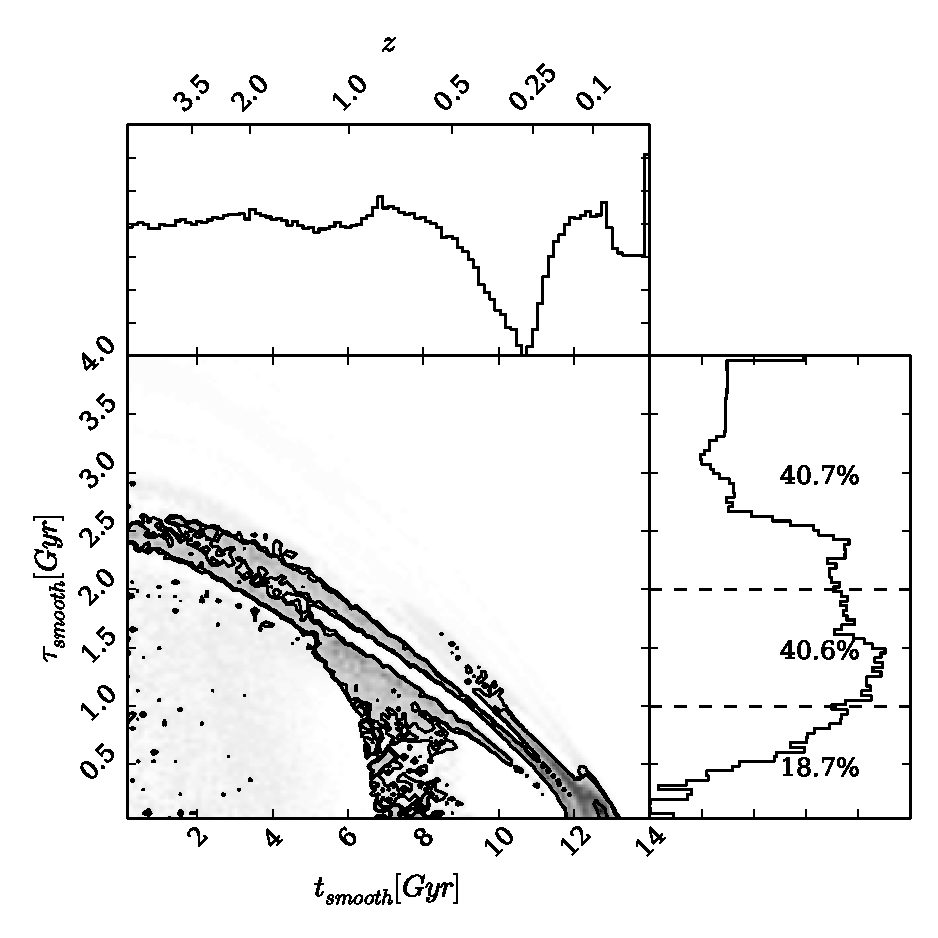
\includegraphics[width=0.4975\textwidth]{morphology/green_smooth.pdf}
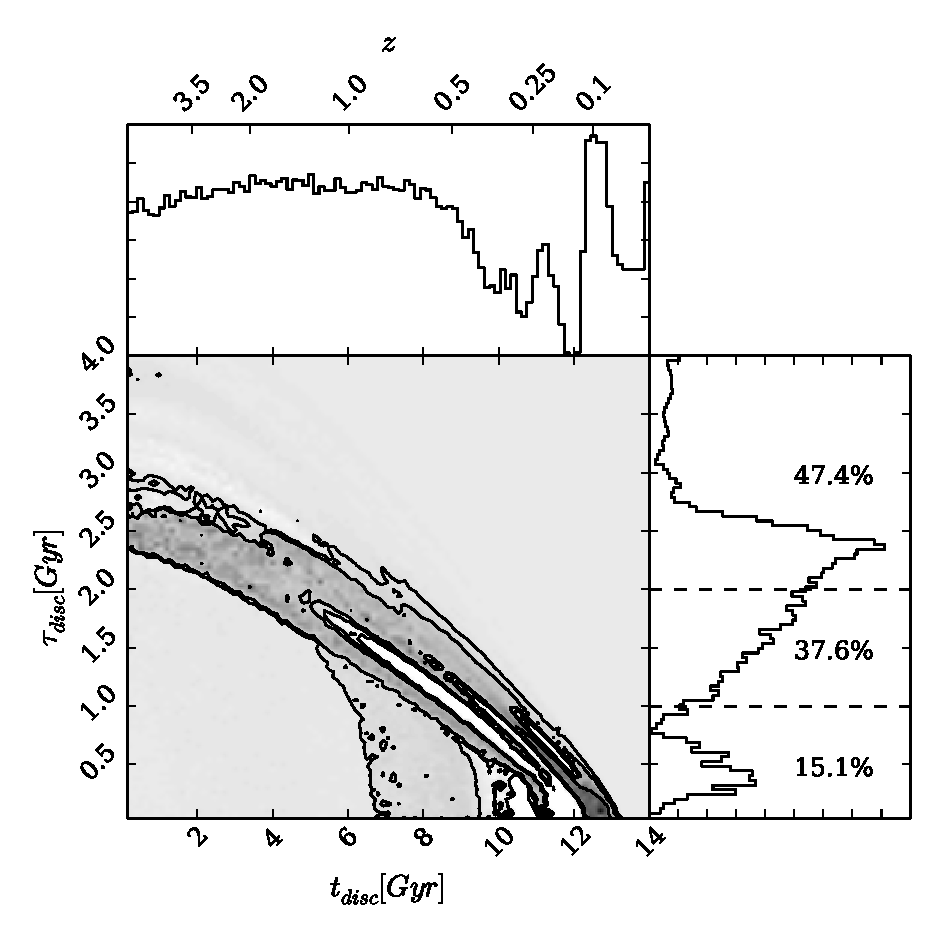
\includegraphics[width=0.4975\textwidth]{morphology/green_disc.pdf}
\caption[Population densities of green smooth and disc galaxies]{Contour plots showing the combined positions in the Markov Chain for galaxies in the green valley, weighted by the logarithmic probability of each position (see Section \ref{stats}) and also by the morphological vote fractions from GZ2 to give the areas of high probability in the model parameter space for both bulge (left) and disc (right) dominated systems. The histograms show the projection into one dimension for each parameter. The dashed lines show the separation between rapid ($\tau ~\rm{[Gyr]} < 1.0$), intermediate ($1.0 < \tau ~\rm{[Gyr]} < 2.0$) and slow ($\tau ~\rm{[Gyr]} > 2.0$) quenching timescales with the fraction of the combined posterior probability distribution in each region shown (see Section~\ref{stats}).}
\label{green_v}
\end{figure*}

In Figure~\ref{green_v} we can make similar comparisons for the green valley galaxies to those discussed previously for the subset of red galaxies studied. For the red galaxies, an argument can be made for two possible tracks across the green valley, shown by the bimodal nature of both distributions in $\tau$ with a common area in the intermediate timescales region where the rapid and slow timescales peaked distributions intersect. However in the green valley this intermediate quenching timescale region becomes more significant  (in agreement with the conclusions of \citealt{Gonc12}), particularly for the smooth-like galaxies (see the left panel of Figure~\ref{green_v}).

The smooth galaxy parameters favour these intermediate quenching timescales ($40.6\%$) with some preference for slow quenching at  early times ($z > 1$). The preference for rapid quenching of smooth galaxies has dropped by over a half compared to the red galaxies, however this will be influenced by the observability of galaxies undergoing such a rapid quench which will spend significantly less time in the transitional population of the green valley. Those galaxies with such a rapid decline in star formation will pass so quickly through the green valley they will be detected at a lower number than those galaxies which have stalled in the green valley with intermediate quenching timescales; accounting for the observed number of intermediate galaxies which are present in the green valley and the dominance of rapid timescales detected for red galaxies for both morphologies.

The disc galaxies of the green valley now overwhelmingly prefer slow quenching timescales ($47.4\%$) with a similar amount of intermediate quenching compared to the smooth galaxy parameters ($37.6\%$; see Figure~\ref{green_v}). There is still some preference for galaxies with a star formation history which results in a high current SFR, suggesting there are also some late-type galaxies that have just progressed from the blue cloud into the green valley. 

If we compare Figure~\ref{green_v} to Figure~\ref{red_s}  we can see quenching has occurred at later (more recent) cosmic times in the green valley at least for red galaxies for both morphological types. Therefore both morphologies are tracing the evolution of the red sequence, confirming that the green valley is indeed a transitional population between blue cloud and red sequence regardless of morphology. Currently as we observe the green valley, its main constituents are very slowly evolving disc-like galaxies along with intermediate- and smooth-like galaxies which pass across it with intermediate timescales within $\sim 1.0-1.5~\rm{Gyr}$.

Given enough time ($t\sim4 - 5~\rm{Gyr}$), the disc galaxies will eventually fully pass through the green valley and make it out to the red sequence (the right panel of Figure~\ref{sfr_mass_col} shows galaxies with $\tau > 1.0~\rm{Gyr}$ do not approach the red sequence within $3~\rm{Gyr}$ post quench). This is most likely the origin of the `red spirals'.

If we consider then that the green valley is a transitional population, then we can expect that the ratio of smooth:disc galaxies that is currently observed in the green valley will evolve into the ratio observed for the red galaxies with NUV emission investigated. Table~\ref{subs} shows the ratio of smooth : disc galaxies in the observed red sequence of the GZ2 sample is $62:38$ whereas in the green valley it is $45:55$. Making the very simple assumptions that this ratio does not change with redshift and that quenching is the only mechanism which causes a morphological transformation, we can infer that $31.2\%$ of the disc-dominated galaxies currently residing in the green valley would have to undergo a morphological change to a bulge-dominated galaxy. We find that the fraction of the probability for green valley disc galaxies occupying the parameter space $\tau < 1.5 ~\rm{Gyr}$ is $29.4\%$, and therefore suggest that quenching mechanisms with these timescales are capable of destroying the disc-dominated nature of galaxies. This is most likely an overestimate of the mechanisms with timescales that can cause a morphological change because of the observability of those galaxies which undergo such a rapid quench; \citet{Martin07} showed that after considering the time spent in the green valley, the fraction of galaxies undergoing a rapid quench quadruples.

All of this evidence suggests that there are not just two routes for galaxies through the green valley as concluded by S14, but a continuum of quenching timescales which we can divide into three general regimes: rapid ($\tau < 1.0 ~\rm{Gyr}$), intermediate ($1.0 < \tau < 2.0~\rm{Gyr}$) and slow ($\tau > 2.0~\rm{Gyr}$). The intermediate quenching timescales reside in the space between the extremes sampled by the UV/optical diagrams of S14; the inclusion of the intermediate galaxies in this investigation (unlike in S14) and the more precise Bayesian analysis, quantifies this range of $\tau$ and specifically ties the intermediate timescales to all variations of galaxy morphology.


\section{Blue Cloud Galaxies}\label{bc}

\begin{figure*}
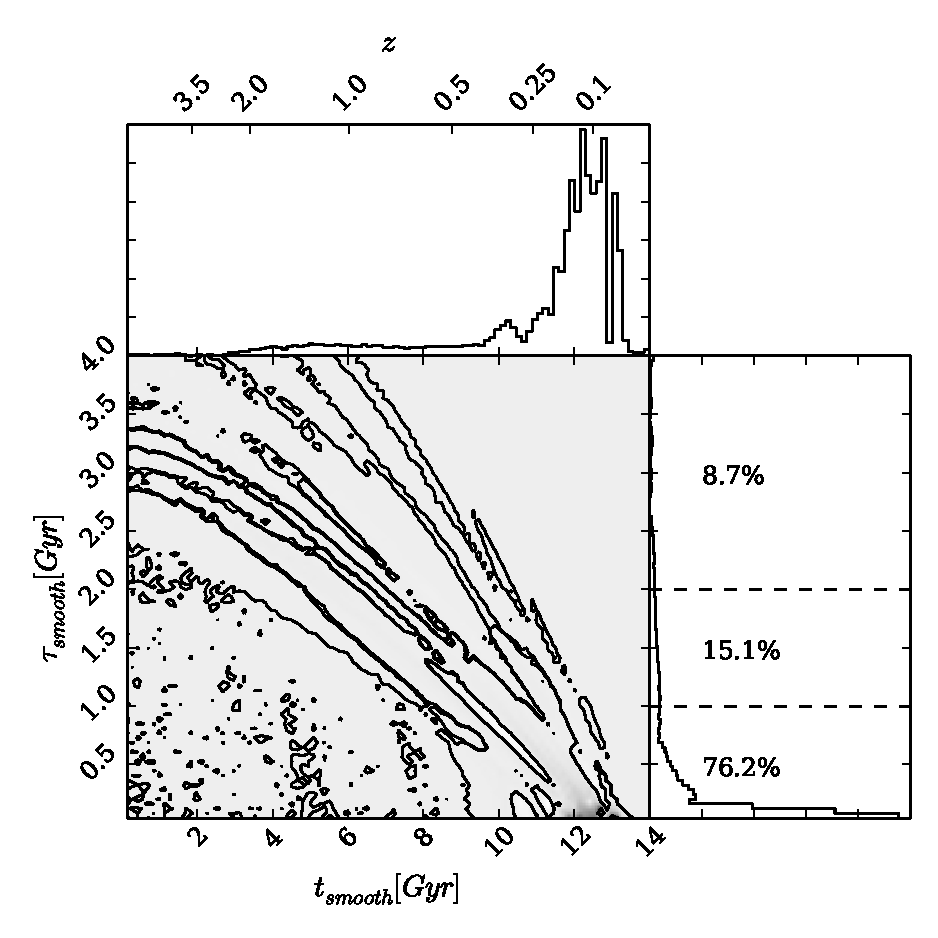
\includegraphics[width=0.4975\textwidth]{morphology/blue_smooth.pdf}
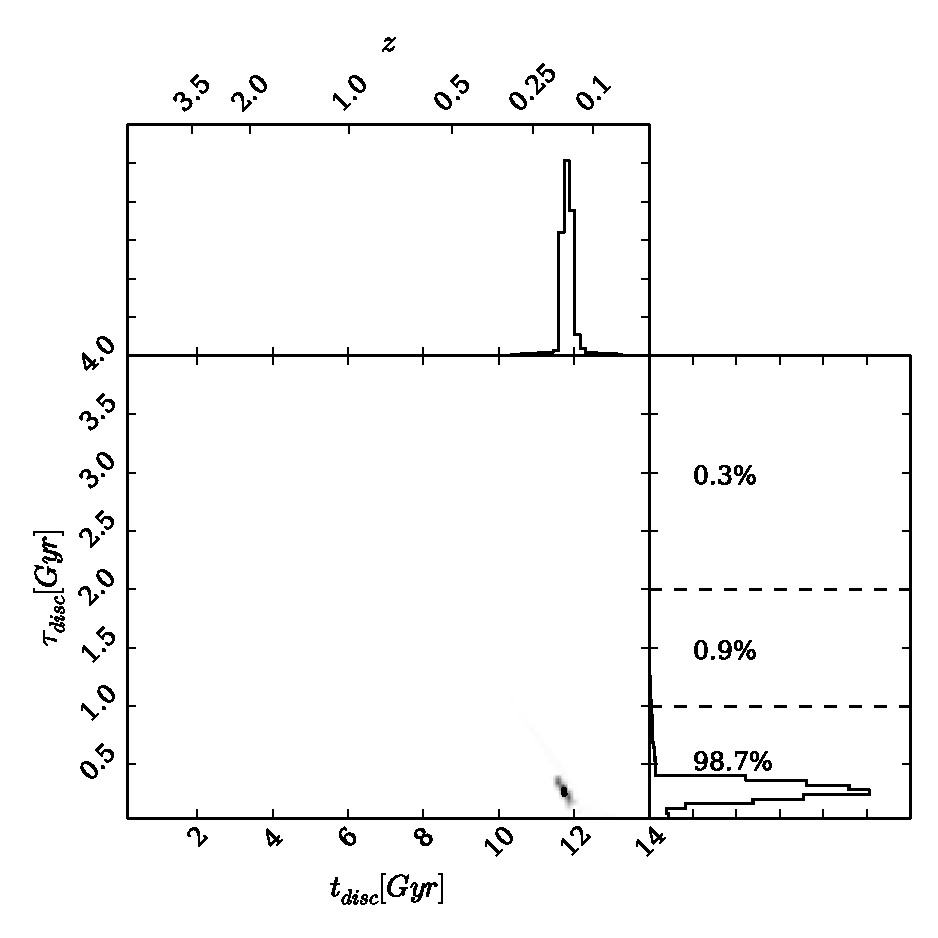
\includegraphics[width=0.4975\textwidth]{morphology/blue_disc.pdf}
\caption[Population densities of blue smooth and disc galaxies]{Contour plots showing the combined positions in the Markov Chain for galaxies in the blue cloud, weighted by the logarithmic probability of each position (see Section \ref{stats}) and also by the morphological vote fractions from GZ2 to give the areas of high probability in the model parameter space for both bulge (left) and disc (right) dominated systems. The histograms show the projection into one dimension for each parameter. The dashed lines show the separation between rapid ($\tau ~\rm{[Gyr]} < 1.0$), intermediate ($1.0 < \tau ~\rm{[Gyr]} < 2.0$) and slow ($\tau ~\rm{[Gyr]} > 2.0$) quenching timescales with the fraction of the combined posterior probability distribution in each region shown (see Section~\ref{stats}). Positions with probabilities less than 0.2 are discarded as poorly fit models, therefore we can conclude unsurprisingly that blue cloud galaxies are not well described by a quenching star formation model. }
\label{blue_c}
\end{figure*}

\begin{figure*}\label{bestfit}
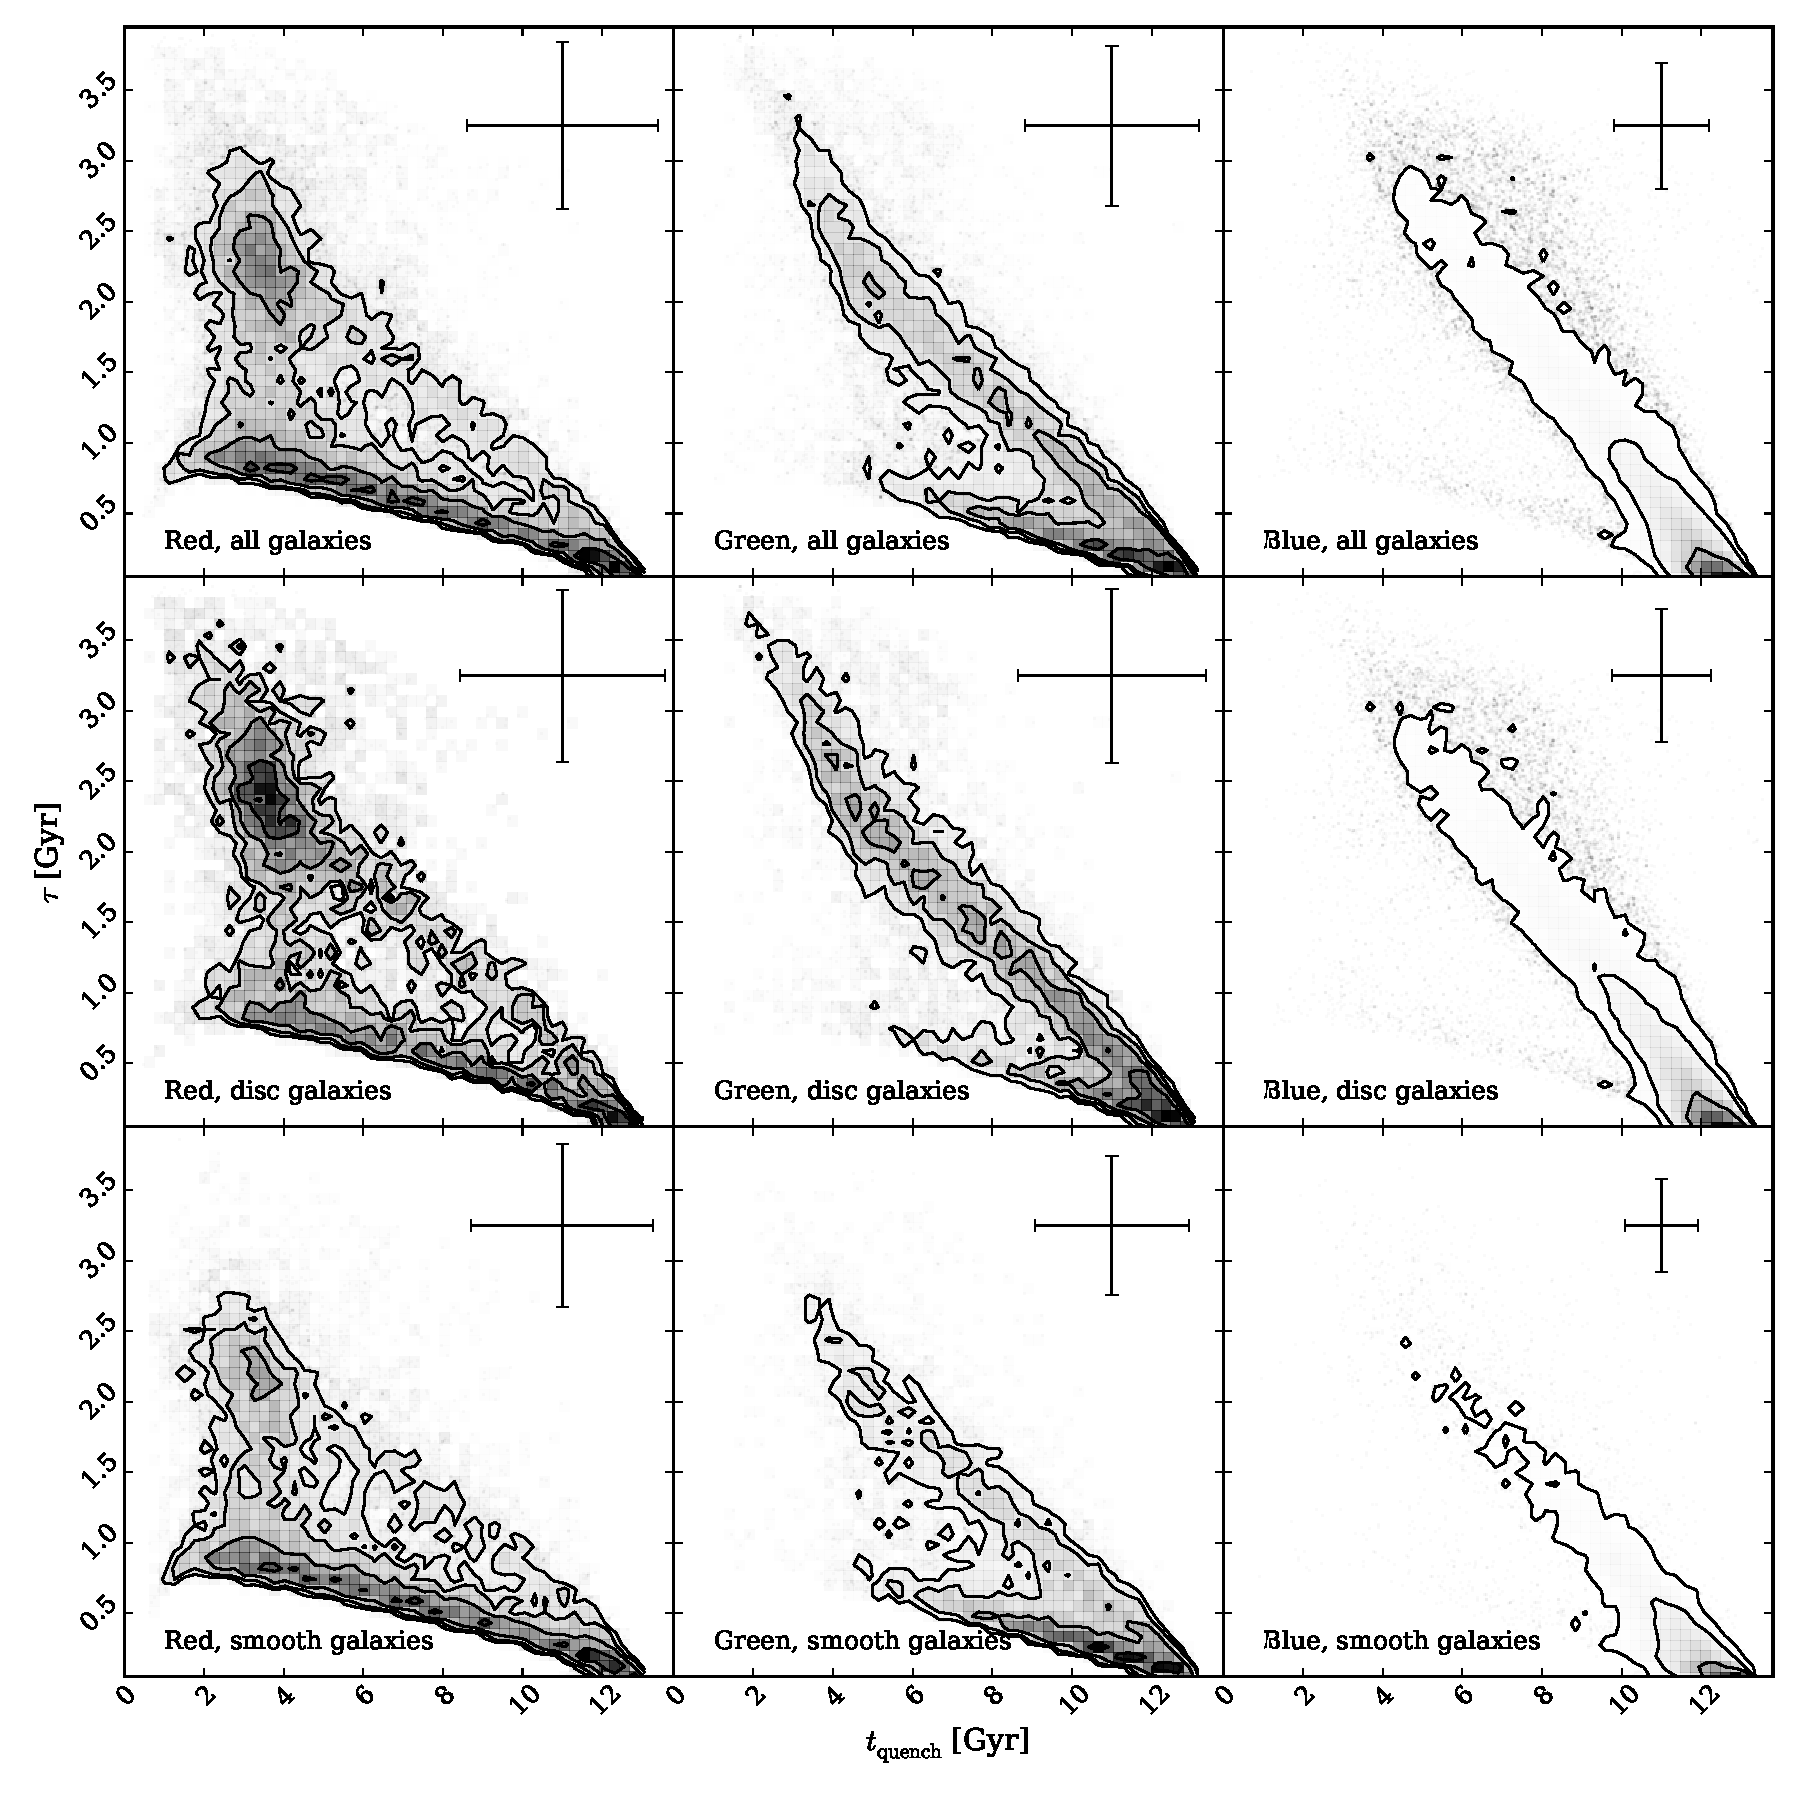
\includegraphics[width=0.95\textwidth]{morphology/contour_t_tau_mcmc_bestfit.pdf}
\caption[Best fit contours for red, green and blue clean galaxies]{Contours showing the positions in the $[t, \tau]$ parameter space of the median walker position (the 50th percentile; as shown by the intersection of the solid blue lines in Figure~\ref{one_example}) for each galaxy for all (top), disc ($p_d > 0.5$; middle), and smooth ($p_s > 0.5$; bottom) red sequence, green valley and blue cloud galaxies in the left, middle and right panels respectively. The error bars on each panel shows the average $68\%$ confidence on the median positions (calculated from the 16th and 84th percentile, as shown by the blue dashed lines in Figure~\ref{one_example}). These positions were calculated without discarding any walker positions due to low probability and without weighting by vote fractions, therefore this plot may be more intuitive than Figures~\ref{red_s},~\ref{green_v} \&~\ref{blue_c}. The differences between the smooth and disc populations and between the red, green and blue populations remain clearly apparent.}
\end{figure*}

Since the blue cloud is considered to be primarily made of star forming galaxies we expect \starpy~ to have some difficulty in determining the most likely quenching model to describe them, as confirmed by Figure~\ref{blue_c}. The attempt to characterise a star forming galaxy with a quenched SFH model leads \starpy~ to attribute the extremely blue colours of the majority of these galaxies to fast quenching at recent times (i.e. very little change in the SFR; see the right panel of Figure~\ref{blue_c} in comparison with the bottom panel of Figure~\ref{pred}).

This is particularly apparent for the blue disc population. Perhaps even galaxies which are currently quenching slowly across the blue cloud cannot be well fit by the quenching models implemented, as they still have high SFRs despite some quenching (although a galaxy has undergone quenching, star formation can still occur in a galaxy, just at a slower rate than at earlier times, described by $\tau$).


There is a very small preference among blue bulge dominated galaxies for slow quenching which began prior to $z \sim 0.5 $. These populations have been blue for a considerable period of time, slowly using up their gas for star formation by the Kennicutt$-$Schmidt law \citep{Schmidt59, Kennicutt97}. However the major preference is for rapid quenching at recent times in the blue cloud; this therefore provides some support to the theories for blue ellipticals as either merger-driven ($\sim76\%$; like those identified as recently quenched ellipticals with properties consistent with a merger origin by \citealt{McIntosh14}) or gas inflow-driven reinvigorated star formation that is now slowly decreasing ($\sim24\%$; such as the population of blue spheroidal galaxies studied by \citealt{Kaviraj13}). However, we remind the reader that the quenching models used in this work do not provide an adequate fit to the blue cloud population.

The blue cloud is therefore primarily composed of both star forming galaxies with any morphology and smooth galaxies which are undergoing a rapid quench, presumably after a previous event triggered star formation and turned them blue.

